%% !Mode:: "TeX:UTF-8"
\documentclass{mcmthesis}
%  \documentclass[CTeX = true]{mcmthesis}
\mcmsetup{tstyle=\color{red}\bfseries,%修改题号,队号的颜色和加粗显示,黑色可以修改为 black
        tcn = 2512625, problem = C, %修改队号,参赛题号
        sheet = true, titleinsheet = true, keywordsinsheet = true,
        titlepage = false, abstract = true}

% 代码块设置
    \usepackage{fontspec}
    \setmainfont{Charter} [
        Extension = .ttf,
        UprightFont = * Regular,
        BoldFont = * Bold, 
        ItalicFont = * Italic,
        BoldItalicFont = * Bold Italic
    ]
    \newfontfamily\consolasfont{Consola}[
        Extension = .ttf,
        UprightFont = *,
        BoldFont = *b,
        ItalicFont = *i,
        BoldItalicFont = *z
    ]

    \definecolor{bg}{rgb}{0.92,0.95,1.0} % Lighter blue fill
    \definecolor{borderblue}{rgb}{0.4,0.4,1.0} % Blue border
    \definecolor{commentcolor}{rgb}{0.4,0.85,0.4} % Softer green comment color

    \lstset{
        basicstyle=\consolasfont,  % Changed to use Consolas
        backgroundcolor=\color{bg},
        lineskip=1.5pt,
        frame=single,
        framesep=1mm,
        rulecolor=\color{borderblue}, % Blue border
        numbers=left,
        numberstyle=\small\color{gray}, % Changed from \tiny to \small
        keywordstyle=\color{blue},
        commentstyle=\color{green},
        commentstyle=\color{commentcolor}\itshape,
        stringstyle=\color{red},
        showstringspaces=false,
        breaklines=true,  % Ensure lines break within margins
        breakatwhitespace=true, % Allow breaking at whitespace
        prebreak=\raisebox{0ex}[0ex][0ex]{\ensuremath{\hookleftarrow}},
        postbreak=\raisebox{0ex}[0ex][0ex]{\ensuremath{\hookrightarrow}},
        escapeinside={(*@}{@*)},
        literate={-}{{\textendash}}1
    }
 
\usepackage{indentfirst}  %首行缩进,注释掉,首行就不再缩进。
\usepackage{lipsum}
\usepackage{wrapfig} % 图文绕排
\title{Mathematical Model for Prediction of Olympic Medal Counts}
\author{\small \href{https://www.latexstudio.net/}
  {\includegraphics[width=7cm]{mcmthesis-logo}}}
\date{\today}

\begin{document}
\begin{abstract}
    \par 
        SUMMARY HERE

\begin{keywords}
    keyword1; keyword2
\end{keywords}

\end{abstract}
\maketitle
\tableofcontents
\newpage

\section{Introduction}
\subsection{Problem Background}
The Olympic medal table is a key focus for nations and fans, reflecting athletic success and national pride. Predicting medal counts, however, is challenging due to the complex factors involved, such as event types, host country advantages, and the emergence of new competitors. This problem requires developing models exclusively based on the provided datasets, including historical medal tables, event breakdowns, and athlete performance.

Traditional forecasting methods, like OLS regression and Poisson models, struggle with accuracy, particularly for countries with zero or few medals. This problem emphasizes predicting medal breakthroughs for such nations, which demands innovative approaches beyond historical trends.

Key aspects include:
\begin{enumerate}
    \item Exploring the relationship between events and medal distributions.
    \item Examining host country advantages and their influence on results.
    \item Assessing the impact of "great coaches" on medal performance, identifying sports where targeted investment in coaching could make a difference.
    \item Projecting medal counts for the 2028 Los Angeles Olympics, including prediction intervals, while addressing uncertainty and potential breakthroughs for nations without prior Olympic success.
\end{enumerate}

\subsection{Literature Review}

Predicting Olympic medal counts has been a topic of interest for researchers across various fields, including economics, sociology, and sports science. Early studies, such as those by Ball (1972) and Grimes et al. (1974), \cite{1} focused on identifying fundamental socioeconomic and demographic factors that influence a nation's medal count. These studies emphasized the importance of population size and economic resources in determining Olympic success. Subsequent research, including work by Bernard and Busse (2004) and Xun Bian (2005) \cite{2}, further explored the impact of political systems and hosting advantages on medal counts, finding that hosting the Games and having a centrally-planned economy can significantly enhance a country's performance.

Recent advancements in statistical and machine learning techniques have led to more sophisticated models for predicting Olympic medals. Schlembach et al. (2022) \cite{5} applied a two-staged Random Forest model, incorporating a wide range of socioeconomic variables, including GDP, population, and public health indicators. This approach outperformed traditional models and naïve forecasts, demonstrating the potential of machine learning to improve prediction accuracy. Similarly, Forrest et al. (2010) \cite{4} enhanced traditional regression-based models by including additional regressors such as public spending on recreation and the effects of future hosts. These studies highlight the importance of considering multiple factors, including public health crises like COVID-19, in predicting Olympic performance.

Despite significant progress, predicting Olympic medals remains a complex task due to the interplay of numerous factors. It's recommended that future research should focus on incorporating more granular data, such as individual athlete performance and training conditions, to enhance prediction accuracy. Additionally, the use of panel data and advanced machine learning techniques, such as neural networks and ensemble methods, could provide further insights into the determinants of Olympic success. It's also deemed important to address the exogeneity of the total number of medals available and considering cultural factors, such as political freedom and gender equality. Overall, the field has evolved from simple correlation-based models to sophisticated machine learning algorithms, with traditional socioeconomic factors remaining significant predictors of Olympic success.

\subsection{Our Work}

Due to the limitation of usable dataset, we cannot explore many of the aforementioned factors in detail. Instead, we focus on developing a model that predicts Olympic medal counts based on historical data and sport-specific information. Our model has the following features:

\begin{enumerate}
    \item A two-stage model that first predicts the number of medals won by each country in each sport, then aggregates these predictions to estimate the total medal count.
    \item Trains and evaluates multiple models with different underlying algorithms on the same dataset, and use the best-performing model for prediction.
    \item Separates different countries into multiple clusters based on their historical medal counts (in which their comprehensive national power is also embodied \cite{7}), allowing for more accurate predictions for countries with similar overall strengths.
    \item A sensitivity analysis that assesses the impact of different factors on medal counts and identifies key drivers of success. 
\end{enumerate}

\section{Assumptions and Justifications} 

\begin{enumerate}
    \item \textbf{Homogeneity of Athletes}: We assume that athletes within the same country are homogeneous in terms of training, resources, and performance. This assumption simplifies the model by treating all athletes from a country as a single entity, ignoring individual variations.
    \item \textbf{Event Independence}: We assume that the outcomes of different events are independent of each other. This assumption allows us to model each event separately without considering potential correlations between them.
    \item \textbf{Historical Consistency}: We assume that historical trends in medal counts are consistent with future performance. This assumption underlies our prediction model, which relies on past data to forecast future outcomes.
    \item \textbf{Host Country Advantage}: We assume that host countries have a competitive advantage due to factors such as home crowd support and familiarity with the venues. This assumption is supported by previous research on the impact of hosting the Olympics on medal counts.
    
\end{enumerate}

\section{Notations and Definitions}


\section{Data Preprocessing}
% remember to mention some details
% 1. event/sport name changed over the course of time
% 2. some special years like 1906, when an unofficial Olympic Games was held. We need to exclude this year from our analysis.
% 3. event name ambiguity, e.g. 500+ events named "Men" and "Women"
\subsection{Early Attempts: Athlete-based Prediction}
Firstly, we negated the method of making prediction based on the historical data of total medals of countries, which is logically unreasonable and too crude. As the most concrete data offered is all individual Olympic competitors with sport, event and result, it is a quite natural thought to predict the medal counts based on every individual athletes.

\subsection{Current Method: Sport/Event Oriented Data Preprocessing}



\section{Establishing the Model}

SSA \cite{8}, DBO \cite{9}, SCA \cite{10}, SA \cite{11}, PSO \cite{12}, SO \cite{13}, POA \cite{14},  
GWO \cite{15}, IGWO \cite{16}, AVOA \cite{17}, CSA \cite{18}, GTO \cite{19}, NGO \cite{20},  
WSO \cite{21}, CGO \cite{22}, INFO \cite{23}, COA \cite{24}, RIME \cite{25}, KOA \cite{26}, RUN \cite{27}.

\section{Task1 --- Predicting Medal Counts for the 2028 Los Angeles Olympics}
\subsection{Subtask --- Exploring the Relationship Between Event Count and Medal Count}

In this subtask, we investigate the relationship between the number and types of events a country participates in and the number of medals it earns. The analysis is performed using data from the 2024 Olympics, focusing on three primary aspects: visualization, correlation analysis, and interpretation of results.

\subsubsection{Visualization}
To better understand the relationship between event count and medal count, we employed two visualization methods:
\begin{itemize}
    \item \textbf{Scatter Plot}: A scatter plot was created to display the relationship between the number of events a country participates in (event count) and the number of medals it earns (medal count).  
    \item \textbf{Box Plot}: To further analyze the distribution of medal counts across different event count intervals, a box plot was used. This visualization captures the median, interquartile range (IQR), and outliers of medal counts for countries grouped into event count bins. The box plot reveals that countries with higher event participation tend to have a wider distribution of medal counts, suggesting greater variability.
\end{itemize}

    
\begin{figure}[htbp]
    \begin{minipage}[t]{0.5\textwidth}
        \centering
        \includegraphics[width=0.8\textwidth]{pics/event_count_vs_medal_count.png}
    \end{minipage}
    \begin{minipage}[t]{0.5\textwidth}
        \centering
        \includegraphics[width=0.9\textwidth]{pics/medal_count_distribution_by_event_count_bins.png}
    \end{minipage}
    \caption{Visualizations: (Left) Scatter plot showing the correlation; 
    (Right) Box plot depicting the distributions.}
\end{figure}

    To better understand the relationship between event count and medal count, countries were grouped into five distinct tiers based on their competitive performance using the K-means clustering algorithm. This method allowed for the segmentation of countries into groups with similar competition characteristics, providing a more nuanced analysis of the underlying relationships.

    The decision to use K-means clustering was motivated by the scatter plot observations, which suggested heterogeneous patterns in the event count and medal count relationship across different types of countries. The clustering process was informed by previous medal achievements(first gold medals, then total medals), ensuring that the grouping reflected meaningful competitive distinctions.
    
    Once the countries were assigned to tiers, we conducted separate correlation analyses within each tier. This approach allowed for a targeted examination of the relationship between event count and medal count, accounting for the differences in competitive capabilities and strategies across tiers. Spearman's correlation coefficient was used to measure the strength and direction of the relationship, as it is well-suited for non-parametric data and can handle potential non-linearities. The results are shown in following Table.


\begin{table}[h!]
    \centering
    \begin{tabular}{ccc}
    \toprule
    \textbf{Tier} & \textbf{Spearman Correlation} & \textbf{p-value} \\
    \midrule
    1 & 0.38 & $2.16 \times 10^{-5}$ \\
    2 & 0.39 & 0.01 \\
    3 & 0.61 & $4.99 \times 10^{-5}$ \\
    4 & 0.57 & 0.13 \\
    5 & 0.98 & 0.02 \\
    \bottomrule
    \end{tabular}
    \caption{Spearman correlation and p-values across different tiers.}
    \label{tab1}
\end{table}

\subsubsection{Interpretation of Results}
The analysis indicates that for most tiers (1, 2, 4, and 5), there is a statistically significant positive relationship between event count and medal count ($p < 0.05$). This suggests that the number of events a country participates in positively impacts its medal count. For Tier 3, the $p$-value is greater than 0.05, indicating no statistically significant correlation between event count and medal count within this group. This anomaly could be due to specific factors such as high variability in event outcomes or unmeasured country-specific attributes.

The correlation coefficients also show a general trend where the relationship between event count and medal count strengthens as the tier increases. This aligns with the expectation that more competitive countries (higher tiers) are better equipped to convert event participation into medals due to superior resources, training, and athletes.

\subsubsection{Conclusions and Recommendations(Optional)}
The results of this analysis demonstrate the critical importance of event participation in achieving higher medal counts. Based on these findings, we propose the following recommendations for countries aiming to improve their medal counts in the 2028 Los Angeles Olympics:
\begin{itemize}
    \item \textbf{Strategic Participation}: Countries should carefully select events where they have a competitive advantage and allocate resources to maximize medal potential.
    \item \textbf{Investment in Training and Resources}: Especially for lower-tier countries, investing in infrastructure, coaching, and athlete preparation can increase their ability to perform well across a broader range of events.
    \item \textbf{Focus on Key Events}: Higher-tier countries should focus on optimizing performance in key events where they historically perform well, while also expanding into new events with medal potential.
\end{itemize}
This analysis underscores the interplay between event participation and medal success, offering actionable insights for Olympic planning and preparation.

\subsection{Subtask --- Identifying the Most Important Sports for Various Countries}

This subtask aims to determine the most significant sports for different countries based on their historical performance in the Olympics. To achieve this, we develop a method to calculate the importance of each event and sport, both at the country level and globally. 

\subsubsection{Notations and Definitions}
Let us define the following notations for the analysis:
\subsubsection{Notations and Definitions}

To facilitate the analysis, we define the key notations in Table~\ref{tab:notations}:


\begin{table}[h!]
    \centering
    \begin{tabular}{@{}ll@{}}
        \toprule
        \textbf{Notation} & \textbf{Definition} \\ 
        \midrule
        $C_i$ & Country $i$, $i \in \{1, 2, \ldots, N\}$; $N$: total number of countries. \\
        $E_j$ & Event $j$, $j \in \{1, 2, \ldots, M\}$; $M$: total number of events. \\
        $S_k$ & Sport $k$, composed of related events $E_j$, \\
             & $k \in \{1, 2, \ldots, L\}$; $L$: total number of sports. \\
        $m_{i,j}$ & Medals won by country $C_i$ in event $E_j$ from 2012 to 2024. \\
        $M_i$ & Total medals won by country $C_i$, \\
             & $M_i = \sum_{j=1}^M m_{i,j}.$ \\
        $w_{i,j}$ & Importance of event $E_j$ for country $C_i$, \\
             & $w_{i,j} = \frac{m_{i,j}}{M_i}.$ \\
        $W_j$ & Global importance of event $E_j$, \\
             & $W_j = \sum_{i=1}^N w_{i,j}.$ \\
        $W_k$ & Global importance of sport $S_k$, \\
             & $W_k = \sum_{j \in S_k} W_j.$ \\
        \bottomrule
    \end{tabular}
    \caption{Notations and their definitions for sports importance analysis.}
    \label{tab:notations}
\end{table}

\subsubsection{Methodology}
To answer the question of which sports are most important for various countries, we proceed with the following steps:

\paragraph{Step 1}

For each country $C_i$ and each event $E_j$, we compute the event importance value $w_{i,j}$ as follows:
\[
w_{i,j} = \frac{m_{i,j}}{M_i}.
\]
This ensures that the sum of importance values for all events for a given country satisfies $\sum_{j=1}^M w_{i,j} = 1$.

\paragraph{Step 2}
For each event $E_j$, we calculate its global importance value $W_j$ as the sum of its importance values across all countries:
\[
W_j = \sum_{i=1}^N w_{i,j}.
\]
This metric captures the relative importance of the event across all countries, regardless of individual country performance.

\paragraph{Step 3}
For each sport $S_k$, we compute its global importance $W_k$ by aggregating the global importance values $W_j$ of all events $E_j$ under the sport:
\[
W_k = \sum_{j \in S_k} W_j.
\]
This step provides an overall measure of the importance of each sport for all countries collectively.

\newpage

\begin{wrapfigure}{r}{8cm}  %这是图文混排的环境
    \centering
    \includegraphics[width=0.9\linewidth,height=10cm]{pics/sport_influence_whole.png}
    \caption{Ranking of sports by global importance based on aggregated event importance values across all countries.}
    \label{fig:sport_importance}
\end{wrapfigure}



\paragraph{Step 4}
The sports are then ranked based on their global importance values $W_k$. A visualization of the rankings illustrates that athletics, boxing, and wrestling are the top three most important sports globally, where athletics has the abosolute highest(more than twice of the second place) importance value.

\subsubsection{Results and Insights}
The analysis reveals that the importance of sports varies significantly across countries. The ranking of sports based on global importance highlights sports such as athletics, swimming, and gymnastics as the most influential globally. These sports typically feature a larger number of events and offer more medal opportunities, which contributes to their higher global importance.

\subsubsection{Discussion and Recommendations}
\begin{itemize}
    \item Countries with limited resources should focus on events with higher importance values $w_{i,j}$ for their specific contexts, as these events offer the best return on investment for medal performance.
    \item Policies that encourage diversification in participation could help countries improve their standings in globally important sports.
    \item Further analysis can include regional comparisons or investigate the temporal trends of sport importance over multiple Olympic cycles.
\end{itemize}


\subsection{Subtask}

\section{Task2 --- The Great Coach Effect: its identification and impact}

The Great Coach Effect is a phenomenon where the presence of a highly skilled coach significantly improves the performance of athletes. Due to the fact that coaches are not bound to a specific country, they can have a significant impact on the medal counts of multiple nations. Identifying the Great Coach Effect and quantifying its impact on medal counts is crucial for predicting Olympic success.

\subsection{Identification}

\subsubsection{Methodology}

We reckon that the Great Coach Effect can be identified by comparing the performance of athletes under the same coach across different countries. It should, by nature, cause one country to have a sharp increase in their medal count in specific sports (otherwise this coach wouldn't be that great), and one other country to go through a gradual-to-sharp decrease in their medal count in the same sports. This is because the coach basically can only focus on coaching one country simultaneously, and the athletes from the other country would not receive the same level of training and support.

Again, due to the inherent limitation of usable dataset, we can only seek to identify the Great Coach Effect from this characteristic, rather than other methods such as relying on coach information to deduce the effect.

Therefore, we propose a two-step approach to identify and quantify the Great Coach Effect:

\begin{enumerate}
    \item Identify such pattern across the dataset.
    \item Refer to outside sources to interpret and cross-verify the result, finding out which specific coach is causing the effect each time.
\end{enumerate}

\subsubsection{Implementation}

We implemented the data filtering logic in Python with 0.23k LOC. The program reads the dataset, groups the data by country, sport, and year, and calculates the weighted medal count for each combination(gold medals with weight 3, silver with 2 and bronze with 1). It then uses linear regression on the most recent 12 years of data to calculate the slope of the medal trend over time. A positive slope exceeding a defined threshold (POS\_K\_LOWER) indicates a sharp increase, while a negative slope below another threshold (NEG\_K\_UPPER) indicates a gradual-to-sharp decrease. Countries with significant trends are recorded as having possible increases or decreases.

The program then pairs countries with overlapping trends in the same sport, checking the overlap period to ensure it spans at least four years and does not exceed a defined gap (OVERLAP\_GAP\_UPPER). Paired trends suggest the transfer of coaching expertise from one country to another.

By carefully calibrating the thresholds and gaps, we can effectively identify the Great Coach Effect and quantify its impact on national performances.

\begin{figure}[htbp]
    \begin{minipage}[t]{0.5\textwidth}
        \centering
        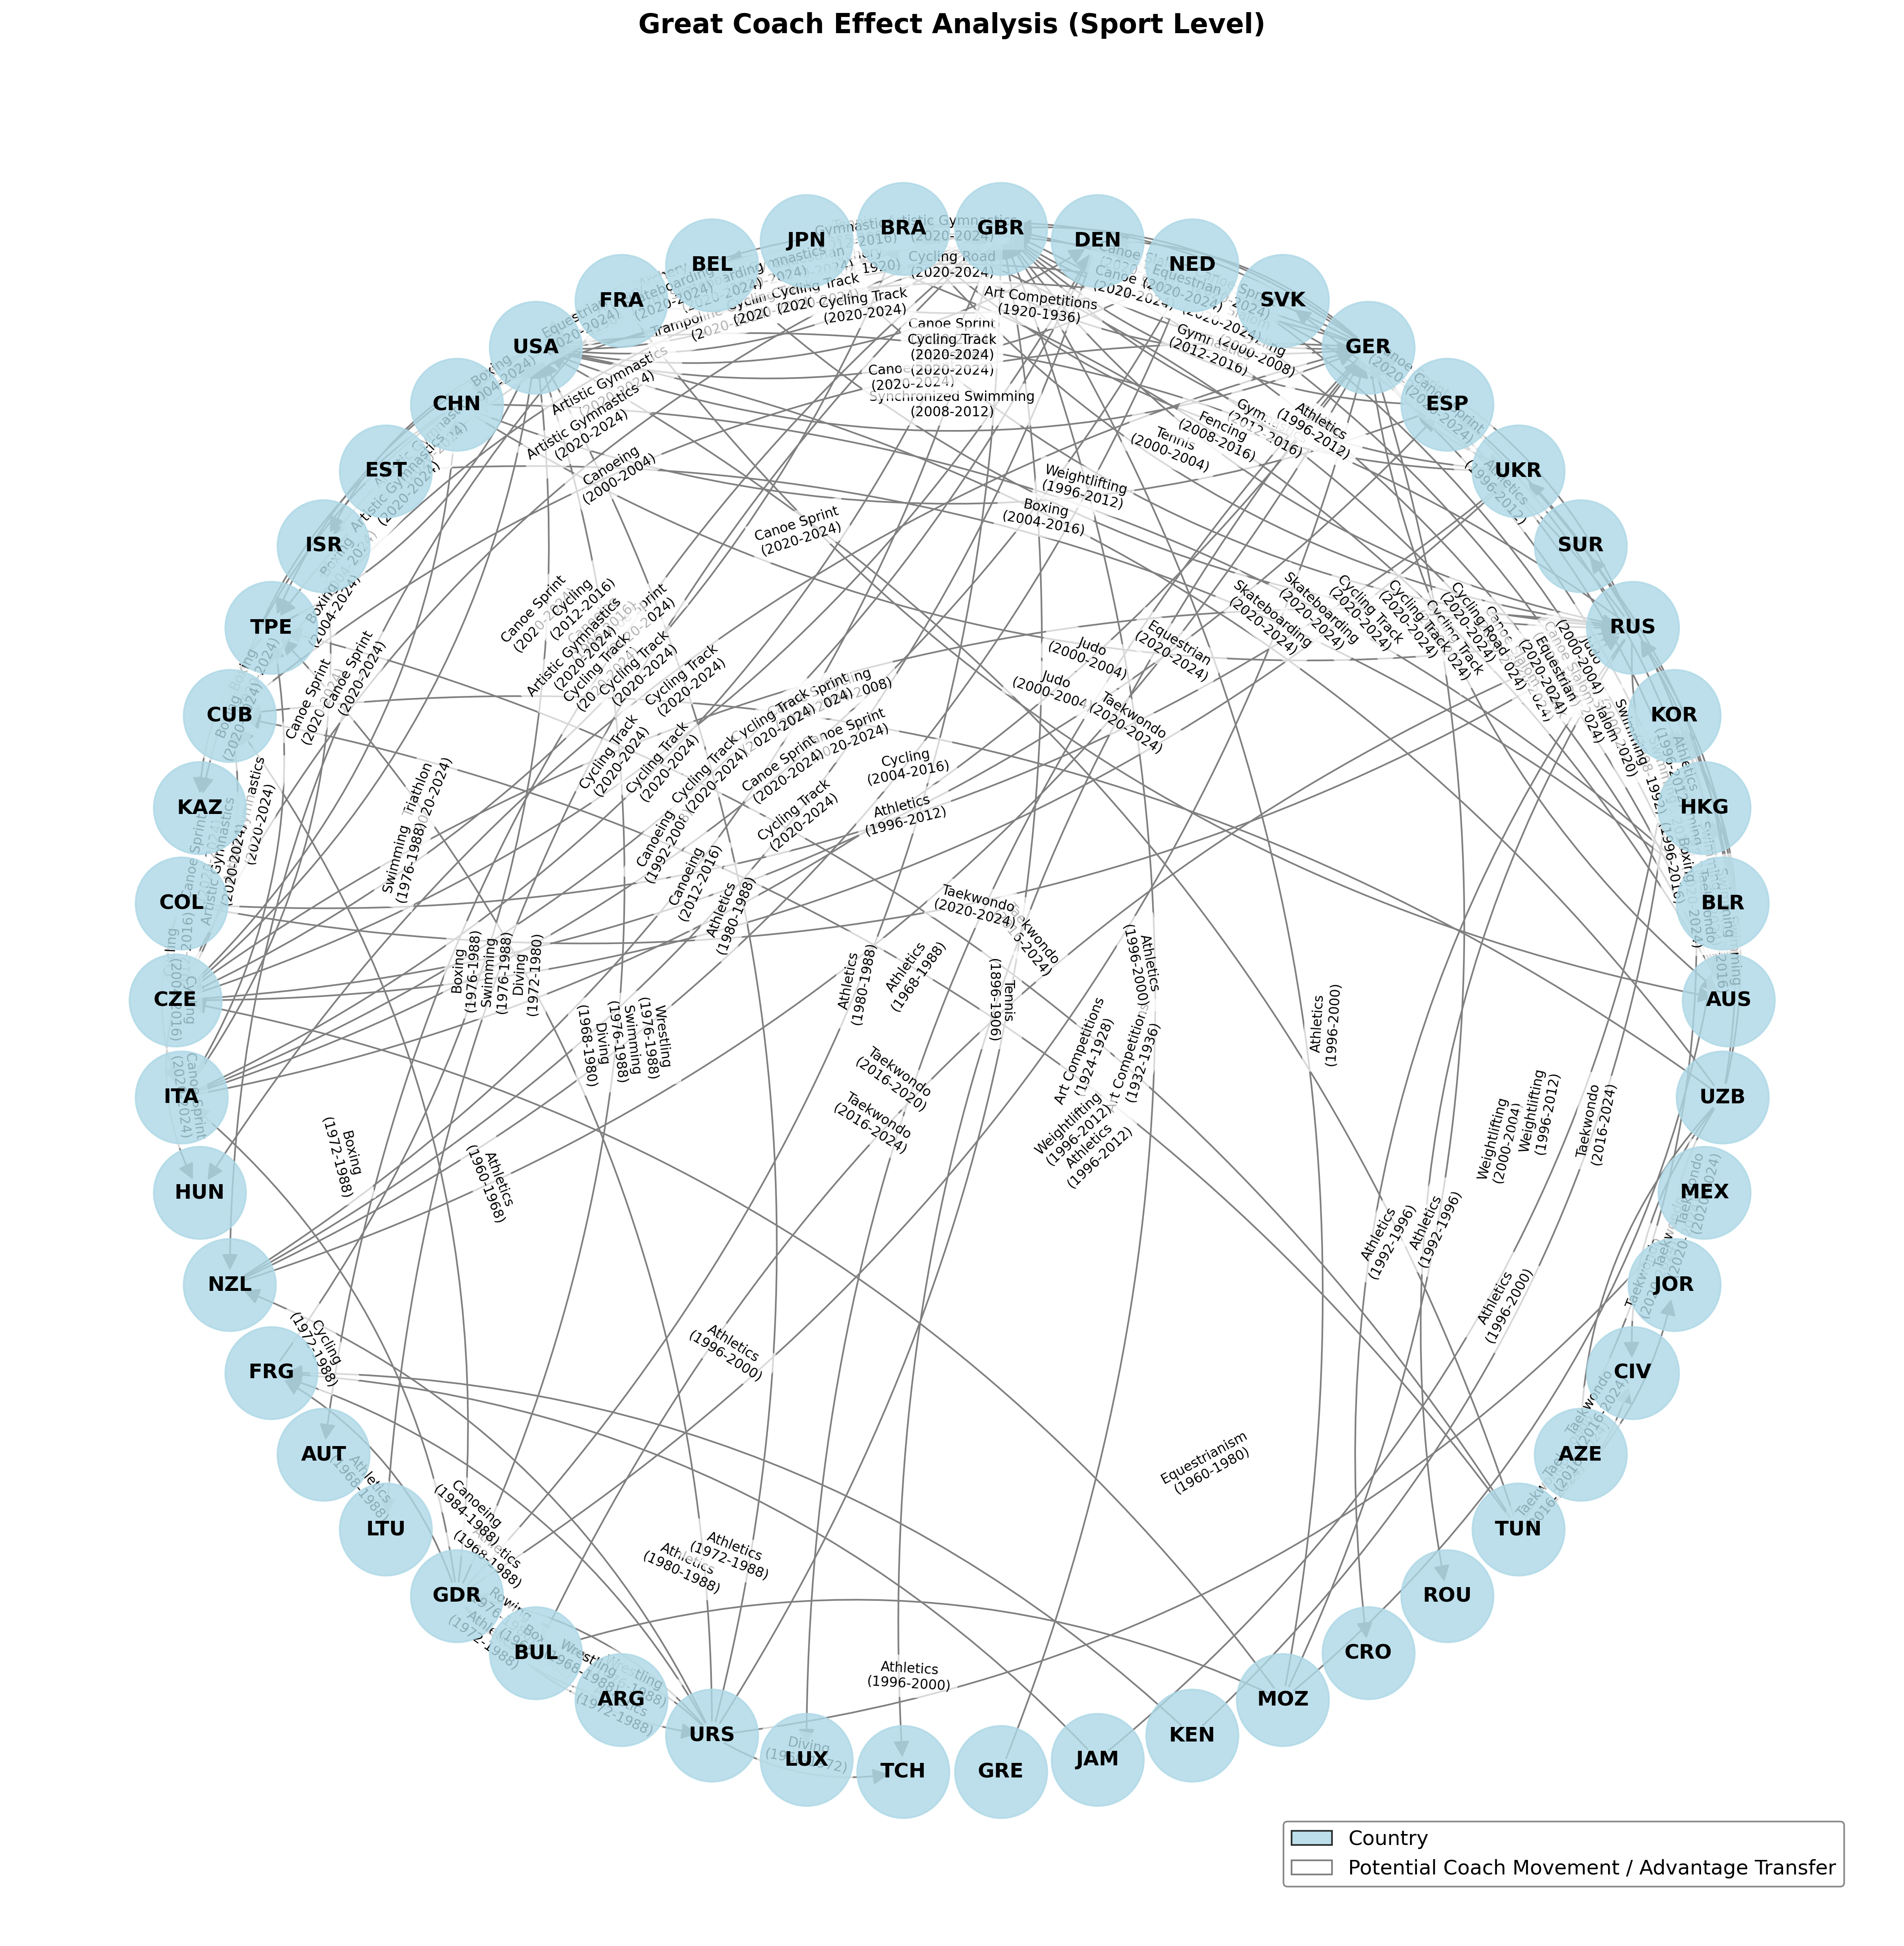
\includegraphics[width=0.8\textwidth]{pics/great_coach_effect_analysis_(sport_level).png}
    \end{minipage}
    \begin{minipage}[t]{0.5\textwidth}
        \centering
        \includegraphics[width=0.8\textwidth]{pics/great_coach_effect_analysis_(event_level).png}
    \end{minipage}
    \caption{Potential occurences of The Great Coach Effects from sport level and event level}
\end{figure}

However elaborate we may calibrate the parameters, there still exists the issue of false positives and false negatives, with false positives accounting more because other factors may also contribute to this same characteristic. We recommend cross-referencing the results with external sources, such as coaching records and athlete interviews, to validate the findings and pinpoint the specific coaches responsible for these shifts. This data-driven approach allows for systematic identification of the Great Coach Effect, providing actionable insights into the strategic importance of coaching in achieving Olympic success.

\subsection{Quantification}

\subsubsection{Methodology}

We will quantify two main aspects of the Great Coach Effect: the magnitude of the performance change in both medal counts changes and the percentage of that change to the total medal count of the country.

The magnitude of the performance change can be calculated by comparing the average medal count before and after the coach transfer, while the percentage of the change can be calculated by dividing the change in medal count by the total medal count of the country in the respective sport.

These two aspects, especially the percentage of medal change to the total medal count of the country, have inextricable correlations with the overall strength of the country. Therefore, we will employ the same strategy as in our model establishment to cluster countries based on their historical medal counts, and then quantify the Great Coach Effect within each cluster.


\subsubsection{Implementation}

We further polish the program used in the identification step to calculate the magnitude and percentage of the Great Coach Effect, adding an additional 0.23k LOC. The program categorizes countries based on their tier value, calculates the average increase/decrease in medal count, and computes the average percentage of this change relative to the total medal count of the country. These metrics provide a comprehensive view of the Great Coach Effect's potential impact on different countries and sports.

\begin{figure}[htbp]
    \centering
    \includegraphics[width=0.8\textwidth]{pics/coach_effect_impact_Sport_from_csv.png}
    \caption{Quantification of The Great Coach Effect}
\end{figure}

\begin{table}[htbp]
    \centering
    \begin{tabular}{|c|c|c|c|c|}
        \hline
        Tier & Avg. Increase & Avg. Decrease & Relative Increase(\%) & Relative Decrease(\%) \\
        \hline
        1 & 1.8125 & -1.6667 & 32.0772 & -10.9944 \\
        \hline
        2 & 2.0562 & -1.6795 & 20.1028 & -9.0563 \\
        \hline
        3 & 2.2623 & -1.9041 & 1.9766 & -0.7317 \\
        \hline
        4 & 2.2743 & -1.7923 & 0.1780 & -0.4518 \\
        \hline
        5 & 2.0746 & -2.4638 & 0.0660 & -0.3472 \\
        \hline
    \end{tabular}
    \caption{Impact of The Great Coach Effect on Different Tiers of Countries}
\end{table}

This figure clearly shows the impact of the Great Coach Effect on different tiers of countries, highlighting the potential for significant performance improvements under the guidance of elite coaches. We can see that the positive and negative impact of the Great Coach Effect(namely, the moving in and out of great coaches) on absolute medal changes has remained constant among different tiers of countries, while its impact on relative medal changes decreases as the tier goes up. This is an expected phenomenon because countries with better overall power already do well in sports across a wide range of fields, so the arrival or departure of one specific coach won't have much effect relative to the total medal count. By quantifying the magnitude and percentage of the effect, we can better understand the strategic value of investing in high-caliber coaching talent and its implications for national Olympic success.

\subsection{Exemplification}
By analyzing the performance trends in specific sports, we identified notable cases where the transfer of a coach coincided with a sharp increase in performance of one country and a decline or stagnation for another, allowing for the cross-verification of our algorithms. Below are three exemplifications of the Great Coach Effect based on historical Olympic data and their correlations with our results.\

It is worth mentioning that the data generated by the program above provides pairs of trends where one country's performance in a certain event increases significantly while another decreases over the same period of time. To spot such pattern, we assign each kind of medal with a value and apply linear regression to the data over a certain of range to get the slope, where a positive slope indicates improvement and vice versa.

\subsubsection{Synchronized Swimming Women's Team: Ana Tarré}
\begin{lstlisting}
- Event: Synchronized Swimming Women's Team, Overlap Years [2008-2012], Increase: CHN(slope=0.125) / Decrease: ESP(slope=-0.250)
\end{lstlisting}

This piece of data generated by the program reveals a significant overlap in performance trends between China (CHN) and Spain (ESP) during the period from 2008 to 2012. China's positive slope (0.125) and Spain's negative slope (-0.250) aligns well with Ana Tarré's transition from coaching Spain to China in 2012.

As we gather the data of a longer period, Ana Tarré's influence as a coach is clearly reflected in the medal trends for synchronized swimming. During her tenure with Spain (1996–2012), the team gradually improved, earning higher medals, peaking with a Silver medal in 2008 and a Bronze in 2012. However, after she transitioned to coaching China in 2012, Spain had dropped out of the podium positions since then until 2024, while China experienced a gradual rise, achieving a series of Silver medals and finnaly a Gold medal in 2024. This shift strongly aligns with the Great Coach Effect, as her expertise and strategies appear to have propelled China's team to the top while Spain struggled without her guidance.

\subsubsection{Gymnastics Women's Team All-Around: Béla Károlyi}
\begin{lstlisting}
- Event: Gymnastics Women's Team All-Around, Overlap Years [2000-2008], Increase: USA(slope=0.125) / Decrease: ROU(slope=-0.250)
\end{lstlisting}

According to the program data, the overlap period between Romania (ROU) and the United States (USA) spans from 2000 to 2008. During this time, Romania exhibited a steep negative slope (-0.250), whereas the United States showed a positive one (0.125), which matches the historical narrative of Béla Károlyi's influence.

Béla Károlyi's legendary coaching career demonstrates a clear pattern of the Great Coach Effect. While coaching Romania (1974–1981), he elevated the team to global prominence, culminating in Silver medals in 1976 and 1980. After moving to coach the United States (1981–2016), Romania's performance declined, while the U.S. women's gymnastics team emerged as a dominant force, securing multiple Gold medals, including in 1996, 2012, and 2016. The sharp contrast in medal trends between the two nations during and after his coaching periods highlights his pivotal role in shaping team success.

\subsubsection{Women's Volleyball: Lang Ping}
\begin{lstlisting}
- Event: Volleyball Women's Volleyball, Overlap Years [1992-2004], Increase: CHN(slope=0.175) / Decrease: USA(slope=-0.075)
- Event: Volleyball Women's Volleyball, Overlap Years [2004-2012], Increase: USA(slope=0.250) / Decrease: CHN(slope=-0.375)
\end{lstlisting}

The program identifies two overlapping periods: 1992-2004 and 2004-2012. In both periods, one of CHN/USA rises and the other falls, which closely corresponds to Lang Ping's coaching career.

Looking at Lang Ping's coaching career spanning over 20 years, we can also discover the distinct influence of a capable coach. During her first tenure with China (1995-2005), the team achieved notable successes, including a Gold medal in 2004. After transitioning to coach the U.S. team (2005-2013) which had won few medals in history, U.S. quickly surpassed China and won 2 consecutive Silver medals. When Lang Ping returned to coach China in 2013, the Chinese team quickly regained its dominance with a Gold in 2016. This fluctuation in performance underscores her unique ability to transform teams and highlights the strategic importance of securing top-tier coaching talent.

% These examples illustrate how the transfer of elite coaches can create significant shifts in medal performance across countries, substantiating the Great Coach Effect. The patterns not only validate the causality between coaching expertise and medal counts but also provide insights for national Olympic committees to consider investing in high-caliber coaching for sustained success.

\subsection{Recommendation}

In the Quantification part, we represented that the Great Coach Effect has a consistent impact on the absolute medal count changes across different tiers of countries, while its impact on relative medal count changes decreases as the tier goes up. This suggests that investing in elite coaching talent can yield substantial performance improvements, particularly for countries with lower historical medal counts(represented by low tier).

Therefore, we recommend that national Olympic committees prioritize recruiting and retaining top-tier coaches for tier 2 countries. Tier 1 countries usually have too tight a budget to afford the cost of coaches with great expertise, while it won't be really necessary for tier 3~5 countries to do so because of the low relative effect.

To determine which three tier 2 countries can benefit the most from the Great Coach Effect, we use the python code from Quantification part and modifies it to find the 3 countries with the highest potential for performance improvement. 

\begin{figure}[htbp]
    \centering
    \includegraphics[width=0.8\textwidth]{pics/tier2_top10_absolute_gain.png}
    \caption{Quantification of The Great Coach Effect}
\end{figure}

From the figure above, we recommend the top 3 countries with the highest potential for performance improvement: ISR (Israel), BRN (Bahrain), and VEN (Venezuela), with respective projected medal gain of 5.5, 3.9 and 3.9.

\section{Sensitivity Analysis}

\subsection{Strengths}

\subsection{How to cite?}
bibliography cite use \cite{1}

% AI cite use \AIcite{AI1,AI2,AI3}

\begin{thebibliography}{99}
    
    \bibitem{1} Ball, D. W. (1972). Olympic Games competition: Structural correlates of national success. International Journal of Comparative Sociology, 15, 186–200.
    \bibitem{2} Bernard, A. B., \& Busse, M. R. (2004). Who wins the Olympic Games: Economic resources and medal totals. Review of Economics and Statistics, 86, 414–417.
    \bibitem{3} Bian, X. (2005). Predicting Olympic Medal Counts: The Effects of Economic Development on Olympic Performance. The Park Place Economist, 13, 37-44.
    \bibitem{4} Forrest, D., Sanz, I., \& Tena, J. D. (2010). Forecasting national team medal totals at the Summer Olympic Games. International Journal of Forecasting, 26, 576–588.
    \bibitem{5} Schlembach, C., Schmidt, S. L., Schreyer, D., \& Wunderlich, L. (2022). Forecasting the Olympic medal distribution – A socioeconomic machine learning model. Technological Forecasting \& Social Change, 175, 121314.
    \bibitem{6} Tcha, M., \& Pershin, V. (2003). Reconsidering performance at the Summer Olympics and revealed comparative advantage. Journal of Sports Economics, 4, 216–239.
    \bibitem{7} Bernard A B, Busse M R. Who wins the Olympic Games: Economic resources and medal totals[J]. Review of economics and statistics, 2004, 86(1): 413-417.
    \bibitem{8} Xue, J., \& Shen, B. (2020). A novel swarm intelligence optimization approach: sparrow search algorithm. \textit{Systems Science \& Control Engineering, 8}(1), 22-34.
    \bibitem{9} Xue, J., \& Shen, B. (2023). Dung beetle optimizer: A new meta-heuristic algorithm for global optimization. \textit{The Journal of Supercomputing, 79}(7), 7305-7336.
    \bibitem{10} Mirjalili, S. (2016). SCA: a sine cosine algorithm for solving optimization problems. \textit{Knowledge-Based Systems, 96}, 120-133.
    \bibitem{11} Steinbrunn, M., Moerkotte, G., \& Kemper, A. (1997). Heuristic and randomized optimization for the join ordering problem. \textit{The VLDB Journal, 6}, 191-208.
    \bibitem{12} Zhan, Z. H., Zhang, J., Li, Y., \& Chung, H. S. H. (2009). Adaptive particle swarm optimization. \textit{IEEE Transactions on Systems, Man, and Cybernetics, Part B (Cybernetics), 39}(6), 1362-1381.
    \bibitem{13} Hashim, F. A., \& Hussien, A. G. (2022). Snake Optimizer: A novel meta-heuristic optimization algorithm. \textit{Knowledge-Based Systems, 242}, 108320.
    \bibitem{14} Trojovský, P., \& Dehghani, M. (2022). Pelican optimization algorithm: A novel nature-inspired algorithm for engineering applications. \textit{Sensors, 22}(3), 855.
    \bibitem{15} Mirjalili, S., Mirjalili, S. M., \& Lewis, A. (2014). Grey wolf optimizer. \textit{Advances in Engineering Software, 69}, 46-61.
    \bibitem{16} Nadimi-Shahraki, M. H., Taghian, S., \& Mirjalili, S. (2021). An improved grey wolf optimizer for solving engineering problems. \textit{Expert Systems with Applications, 166}, 113917.
    \bibitem{17} Abdollahzadeh, B., Gharehchopogh, F. S., \& Mirjalili, S. (2021). African vultures optimization algorithm: A new nature-inspired metaheuristic algorithm for global optimization problems. \textit{Computers \& Industrial Engineering, 158}, 107408.
    \bibitem{18} Braik, M. S. (2021). Chameleon Swarm Algorithm: A bio-inspired optimizer for solving engineering design problems. \textit{Expert Systems with Applications, 174}, 114685.
    \bibitem{19} Abdollahzadeh, B., Soleimanian Gharehchopogh, F., \& Mirjalili, S. (2021). Artificial gorilla troops optimizer: a new nature‐inspired metaheuristic algorithm for global optimization problems. \textit{International Journal of Intelligent Systems, 36}(10), 5887-5958.
    \bibitem{20} Dehghani, M., Hubálovský, Š., \& Trojovský, P. (2021). Northern goshawk optimization: a new swarm-based algorithm for solving optimization problems. \textit{IEEE Access, 9}, 162059-162080.
    \bibitem{21} Braik, M., Hammouri, A., Atwan, J., Al-Betar, M. A., \& Awadallah, M. A. (2022). White Shark Optimizer: A novel bio-inspired meta-heuristic algorithm for global optimization problems. \textit{Knowledge-Based Systems, 243}, 108457.
    \bibitem{22} Talatahari, S., \& Azizi, M. (2021). Chaos game optimization: a novel metaheuristic algorithm. \textit{Artificial Intelligence Review, 54}(2), 917-1004.
    \bibitem{23} Ahmadianfar, I., Heidari, A. A., Noshadian, S., Chen, H., \& Gandomi, A. H. (2022). INFO: An efficient optimization algorithm based on weighted mean of vectors. \textit{Expert Systems with Applications, 195}, 116516.
    \bibitem{24} Dehghani, M., Montazeri, Z., Trojovská, E., \& Trojovský, P. (2023). Coati Optimization Algorithm: A new bio-inspired metaheuristic algorithm for solving optimization problems. \textit{Knowledge-Based Systems, 259}, 110011.
    \bibitem{25} Su, H., Zhao, D., Heidari, A. A., Liu, L., Zhang, X., Mafarja, M., \& Chen, H. (2023). RIME: A physics-based optimization. \textit{Neurocomputing, 532}, 183-214.
    \bibitem{26} Abdel-Basset, M., Mohamed, R., Azeem, S. A. A., Jameel, M., \& Abouhawwash, M. (2023). Kepler optimization algorithm: A new metaheuristic algorithm inspired by Kepler’s laws of planetary motion. \textit{Knowledge-Based Systems, 268}, 110454.
    \bibitem{27} Ahmadianfar, I., Heidari, A. A., Gandomi, A. H., Chu, X., \& Chen, H. (2021). RUN beyond the metaphor: An efficient optimization algorithm based on Runge Kutta method. \textit{Expert Systems with Applications, 181}, 115079.

\end{thebibliography}

\begin{appendices}

\section{First appendix}

% In addition, your report must include a letter to the Chief Financial Officer (CFO) of the Goodgrant Foundation, Mr. Alpha Chiang, that describes the optimal investment strategy, your modeling approach and major results, and a brief discussion of your proposed concept of a return-on-investment (ROI). This letter should be no more than two pages in length.

\begin{letter}{Dear, Mr. Alpha Chiang}

    \vspace{\parskip}

    Sincerely yours,

    Your friends

\end{letter}

\section{Second appendix}

    % \lstinputlisting[language=C++]{./code/mcmthesis-sudoku.cpp}

\end{appendices}

% AI report begins here
\AImatter
\begin{ReportAiUse}{9}
\bibitem{AI1}



\end{ReportAiUse}

\end{document}
